\chapter{Results}

XXXXXXXXXXXXXXXXX

\begin{figure}[ht]
    \centering
    \scalebox{1.2}{

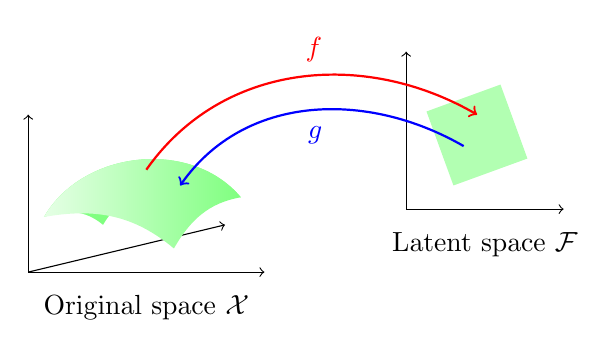
\begin{tikzpicture}
\centering
\draw[->] (0, 0) -- ++(0, 2);
\draw[->] (0, 0) -- ++(2.5, 0.6);
\draw[->] (0, 0) -- ++(3, 0) node[midway, below, yshift=-0.5em]
    {Original space ${\cal X}$};

\draw[fill=green!50, draw=none, shift={(0.2, 0.7)},scale=0.5]
  (0, 0) to[out=20, in=140] (1.5, -0.2) to [out=60, in=160]
  (5, 0.5) to[out=130, in=60]
  cycle;

\shade[thin, left color=green!10, right color=green!50, draw=none,
  shift={(0.2, 0.7)},scale=0.5]
  (0, 0) to[out=10, in=140] (3.3, -0.8) to [out=60, in=190] (5, 0.5)
    to[out=130, in=60] cycle;

  \draw[->] (4.8, 0.8) -- ++(0, 2);
  \draw[->] (4.8, 0.8) -- ++(2, 0) node[midway, below, yshift=-0.5em]
      {Latent space ${\cal F}$};

  \draw[thin, fill=green!30, draw=none, shift={(5.4, 1.1)}, rotate=20]
    (0, 0) -- (1, 0) -- (1, 1) -- (0, 1) -- cycle;

  \draw[thick,->,red]
    (1.5, 1.3) to [out=55, in=150] node[midway, above, xshift=6pt, yshift=2pt]
    {$f$} (5.7, 2);

  \draw[thick,->,blue] (1.5, 1.3) ++(4.03, 0.3) to [out=150, in=55]
    node[midway, below, xshift=2pt, yshift=-2pt] {$g$} ++(-3.6, -0.5);

\end{tikzpicture}}
    
    \caption[Dimensionality reduction and latent space representation \cite{tikz}.]{\small{Dimensionality reduction and latent space representation: Mapping between the original high-dimensional space ${\cal X}$ and the lower-dimensional latent space ${\cal F}$ using functions $f$ and $g$.}}
    \label{fig:manifold}
\end{figure}


\section{Tables and graphics}

XXXXXXXXXXXXXXXXX

Extend table by \cite{Hernandez-Olivan2021MusicFeatures}

\begin{table}[h]
\centering
\footnotesize
\begin{tabularx}{\textwidth}{|X|X|X|X|X|X|X|X|}
\hline
Year & Authors & Ref. & Algorithm & Input & Method & Supervised? & F-measure SALAMI \\
\hline
2009 & Paulus \& Klapuri & [24] & PK & MFCCs, chromas & Fitness function & No & - \\
2010 & Mauch et al. & [25] & MND1 & MFCCs, Discrete Cepstrum & HMM & No & - \\
2011 & Sargent et al. & [26] & SB-VRS1 & Chords estimation & Viterbi & No & - \\
2012 & Kaiser et al. & [27] & KSP2 & SSM & Novelty measure & No & 0.286 \\
2013 & McFee \& Ellis & [20] & MP2 & MLS & Fisher’s Linear Discriminant & No & 0.317 \\
2014 & Nieto \& Bello & [28] & NB1 & MFCCs + chromas & Checkerboard-like kernel & No & 0.299 \\
2015 & Cannam et al. & [29] & CC1 & Timbre-type histograms & HMM & No & 0.213 \\
2016 & Nieto & [30] & ON2 & Constant-Q Transform Spectrogram & Linear Discriminant Analysis & No & 0.299 \\
2017 & Cannam et al. & [29] & CC1 & Timbre-type histograms & HMM & No & 0.212 \\
2014 & Schlüter et al. & [31] & SUG1 & MLS & CNN & Yes & 0.529 \\
2015 & Grill \& Schlüter & [32] & GS1 & MLS + SSLMs & CNN & Yes & 0.541 \\
2007 & Turnbull et al. & [19] & - & MFCCs, chromas, spectrogram & Boosted Decision Stump & No & 0.378 \\
2011 & Sargent et al. & [34] & - & MFCCs, chromas & Viterbi & No & 0.356 \\
2014 & Ullrich et. al & [22] & - & MLS & CNN & No & 0.465 \\
2015 & Grill \& Schlüter & [4] & - & MLS + SSLMs & CNN & No & 0.523 \\
2015 & Grill \& Schlüter & [5] & - & MLS + PCPs + SSLMs & CNN & No & 0.508 \\
2017 & Hadria \& Peeters & [35] & - & MLS + SSLMs & CNN & No & 0.291 \\
\hline
\end{tabularx}
\caption{Your Caption}
\label{tab:my_label}
\end{table}


\begin{figure}[!ht]
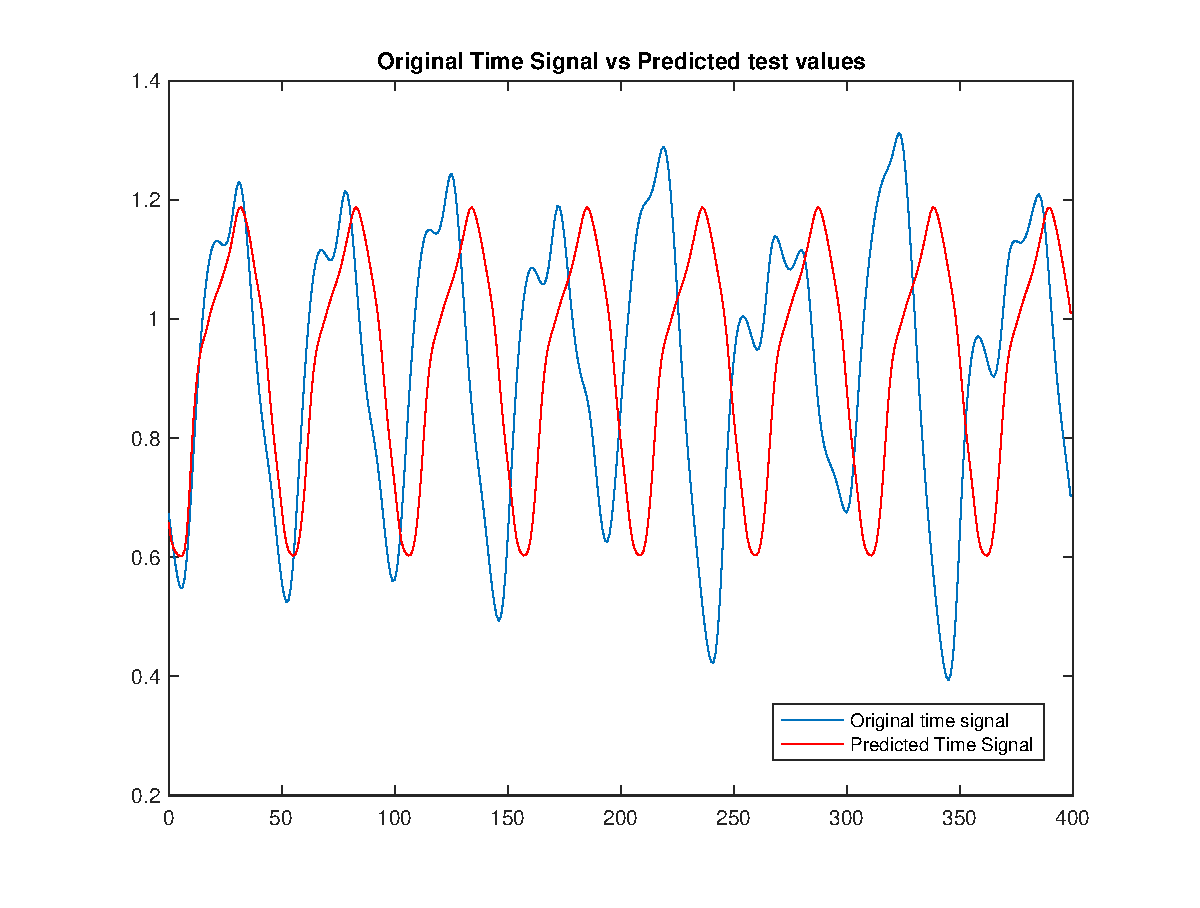
\includegraphics[clip,width=\columnwidth]{figures/PlotTimeSeriesResult}% 
\caption[Graph.]{This is an example of a figure and its caption.}
\label{fig:timeseries}
\end{figure}

\begin{table}[!ht]
\renewcommand{\arraystretch}{1.50}
\caption[Table]{This is an example of a table and its caption.}
\label{tablePCA}
\centering
\begin{tabular}{| c | c | c | c | c |}
\hline
\bfseries PCA & \bfseries Residual mean & \bfseries XXX & \bfseries XXX & \bfseries XXX \\
\hline\hline
Original PCA & 0.1267 & XXX & XXX & XXX  \\
\hline
PCA on Centroid 1 & 0.1249 & XXX & XXX  & XXX\\
\hline
PCA on Centroid 2 & 0.1214  & XXX & XXX  & XXX\\
\hline
\end{tabular}
\end{table}

\newpage


